\documentclass[border=4pt]{standalone}
\usepackage{tikz}
\usetikzlibrary{arrows,arrows.spaced,positioning}
\begin{document}
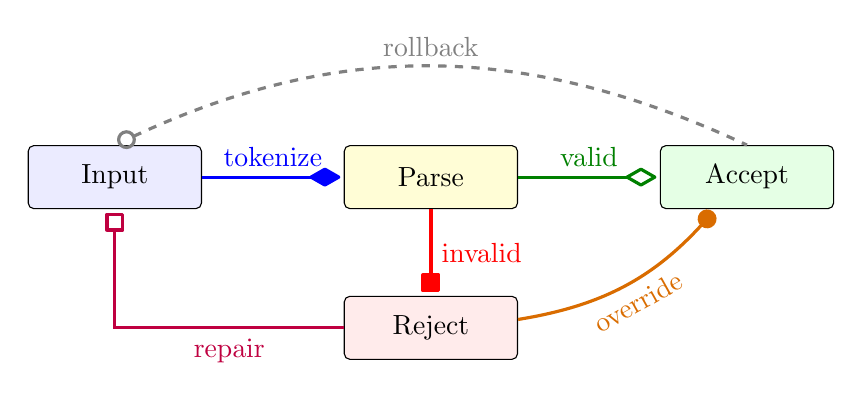
\begin{tikzpicture}[
  node distance=11mm and 18mm,
  stage/.style={draw,rounded corners=2pt,minimum width=22mm,minimum height=8mm,align=center},
  link/.style={line width=1.15pt}
]
  \node[stage,fill=blue!8] (input) {Input};
  \node[stage,fill=yellow!16,right=of input] (parse) {Parse};
  \node[stage,fill=green!10,right=of parse] (accept) {Accept};
  \node[stage,fill=red!8,below=of parse] (reject) {Reject};

  \draw[link,blue,-{spaced diamond}]
    (input) -- node[above]{tokenize} (parse);
  \draw[link,green!50!black,-{spaced open diamond}]
    (parse) -- node[above]{valid} (accept);
  \draw[link,red,-{spaced square}]
    (parse) -- node[right]{invalid} (reject);
  \draw[link,purple,-{spaced open square}]
    (reject.west) -| node[pos=.25,below]{repair} (input.south);
  \draw[link,orange!85!black,-{spaced *}]
    (reject) to[bend right=20] node[below,sloped]{override} (accept);
  \draw[link,dashed,gray,{spaced o}-]
    (input.north) to[bend left=25] node[above,sloped]{rollback} (accept.north);
\end{tikzpicture}
\end{document}
